%%%%%%%%%%%%%%%%%%%%%%%%%%%%%%%%%%%%%%%%%%%%%%%%%%%%%%%%%%%%%%%%%%%%%%%%%%%%%%%%
%2345678901234567890123456789012345678901234567890123456789012345678901234567890
%        1         2         3         4         5         6         7         8
% THESIS CHAPTER


\chapter[Control Architecture: Methods \& Results]{Control Architecture: \\ Methods \& Results}
\label{chap:method}
\ifpdf
    \graphicspath{{Method/Figures/PNG/}{Method/Figures/PDF/}{Method/Figures/}}
\else
    \graphicspath{{Method/Figures/EPS/}{Method/Figures/}}
\fi

\begin{figure}[H]
	\centering
	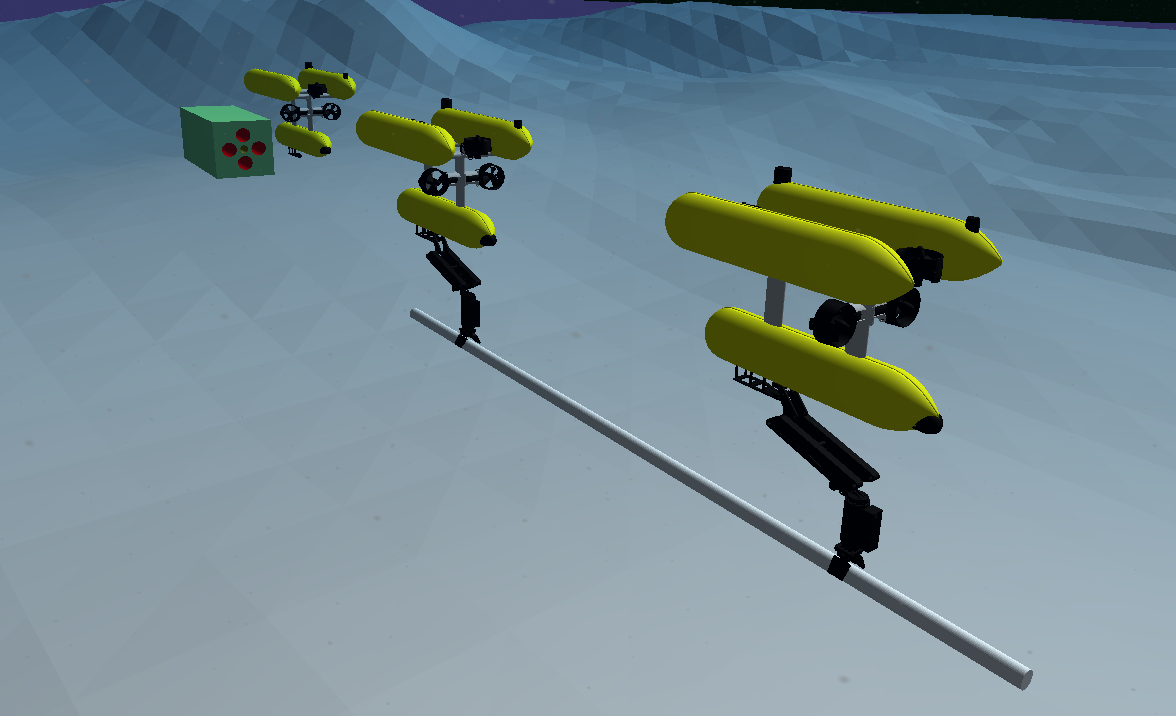
\includegraphics[width=14.5cm]{scenario_whole.png}
	\caption[The Scenario with the two robot carrying the peg and the vision robot watching the hole]{The Scenario of the experiment. The two twin robots are carrying the common peg, while the third robot is watching the hole to estimate its pose.}
	\label{fig:method_uwsim}
\end{figure}

In this chapter, experimental set-up is described, and results are given and discussed. The code for the whole architecture is available at \href{https://github.com/torydebra/AUV-Coop-Assembly}{https://github.com/torydebra/AUV-Coop-Assembly}.\\
%todo and explained a bit in the appendix?

The scenario is made up of two I-AUV's \href{https://cirs.udg.edu/auvs-technology/auvs/girona-500-auv/}{Girona 500 AUV} underwater vehicles, each one equipped with a CSIP Robot arm5E (4 DOF arm with a parallel yaw gripper). The final goal is to successfully coordinate the robots in such a way that the peg, hold by both manipulators, is inserted correctly in the other piece, fixed in the environment. One robot is equipped with a force torque sensor that permits to understand forces applied on the peg, caused during the insertion phase. This information is provided to both robots.

The chosen strategy divides the problem in two phases: Hole Detection and Insertion. In the first preliminary step are done to detect the hole. A third robot, not used for manipulation task, is in charge to exploit vision to estimate the pose of the hole. Detail about this are given in section \ref{chap:vision}.
The second phase explores the problems inherent to the interaction between the peg and the hole, and the communication between the carrying agents. This is described in this chapter.
                          
%todo descrivi la situa: due piu uno robot, il peg, hole nel ambiete. e metti foto per mostrare ste cose

%todo dire in sect 1 blabla... ecc

\section{Simulators}
\label{sec:simulators}
A bit effort has been spent to choice a suitable simulator for the case. At the end, \href{http://www.irs.uji.es/uwsim/}{UWSim} [\cite{uwsim}] was chosen. It is a simulator largely used for this kind of scenarios, which visualize a virtual underwater scene. It provides a different variety of useful sensors (e.g. the used force-torque sensor and the cameras), but also others can be added. It is fully integrate in ROS, which made it really easy to use. ROS is used as simulator interface: through ROS messages, we can send commands to the robots and we can receive information from the going on test. Contact physics is implemented integrating the physics engine \href{https://pybullet.org/wordpress/}{Bullet} with \href{http://www.openscenegraph.org/}{OSG} through \href{https://github.com/mccdo/osgbullet}{OSGBullet}. To further details about how the simulation is implemented, especially the contact physics part, please refers to the documentation of the cited software. The cons in using UWSim is that the simulations is fully kinematic, so no dynamics interaction ar present. This means, for example, that velocity sent to the robot are immediately accomplished, and that we can't simulate the real physics while grasping a real object. For the scope of this thesis, this lack is not important because dynamics is not considered. Furthermore, the only needed dynamic part, i.e. how the contact between the tool and the hole affect the whole manipulator chain, can be simulated at kinematic level thanks to the information provided by the force-torque sensor, as explained in section \ref{sec:forceConsideration}.\\
To fill the lack of dynamic of UWSim, a good alternative can be \href{https://github.com/freefloating-gazebo/freefloating_gazebo}{FreeFloatingGazebo} [\cite{freeFloatingGazebo}]. In truth, this simulator is a plug-in for Gazebo and UWSim; it integrates them in order to achieve both dynamic (thanks to Gazebo) and visually realistic I-AUV simulation (thanks to UWSim). The interface used to communicate with the simulation is the same of UWSim, so ROS and its messages, which make it easy as UWSim to use. \\
This plug-in has been taken into consideration for dynamic test, that are not evaluated due to the lack of time, but can be certainly used for further works.
\href{http://gazebosim.org/}{Gazebo} is a generic simulator widely used in all robotics fields. It is the de-facto simulator for ROS. Seen its purpose, it is not a ready-to use simulator for underwater environment, and can be only a starting point to build a software to simulate this particular scenario (as it is done by FreeFloatingGazebo).\\
Also other simulators, \href{http://www.coppeliarobotics.com/index.html}{V-REP} [\cite{vrep}] and \href{https://cyberbotics.com/}{Webots} [\cite{webots}] have been taken into consideration but discarded for same \enquote{not ready-to-use} reason like Gazebo.\\
An interesting simulator is \href{https://github.com/disaster-robotics-proalertas/usv_sim_lsa}{USV simulator} [\cite{usvsim}] which takes the best from UWSim, Gazebo and FreeFloatingGazebo to implement realistic simulation. This is a really recent and in development project, and however it is focused more on surface vessels dynamics.\\

More details and comparisons are available in \cite{simComparisonCook} and \cite{usvsim}, and a schematic recap taken from \cite{usvsim} is visible in fig. \ref{fig:simComparison}.
\begin{figure}[H]
	\centering
	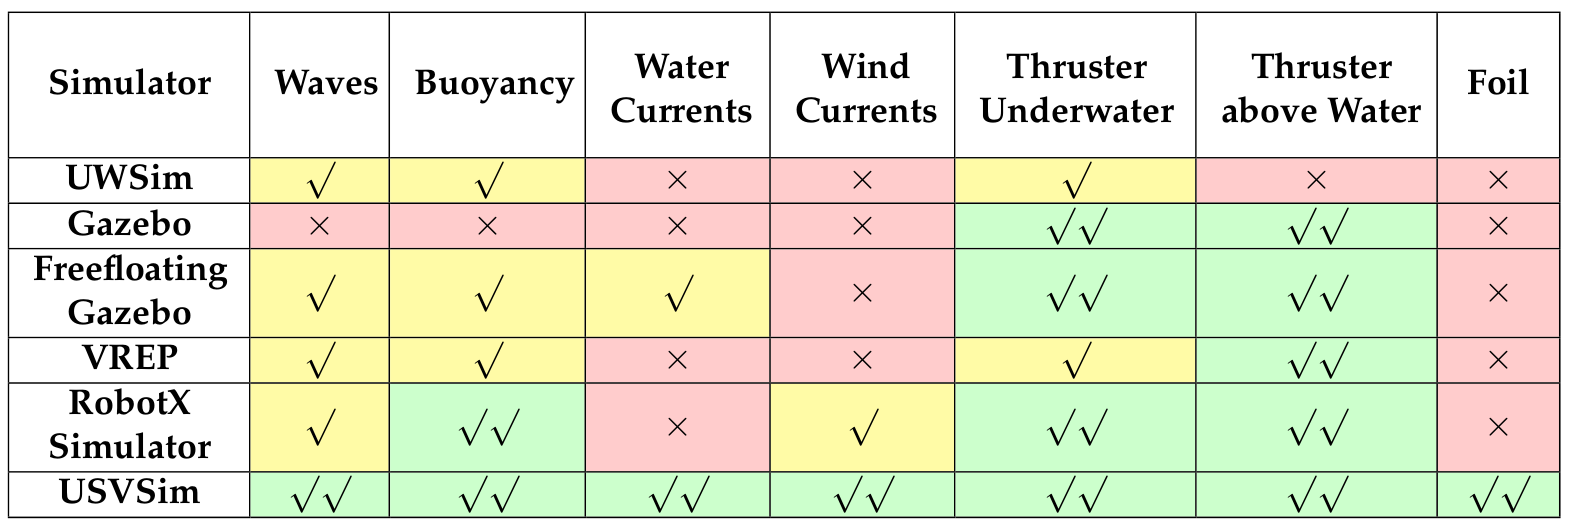
\includegraphics[width=14cm]{simComparison.png}
	\caption[Schematic Simulators Comparison]{Schematic recap of simulation comparison taken from \cite{usvsim}. $\times$ stands for no implemented feature; ~ $\surd\,$  for a feature that is a discrete representation of the real one; ~ $\surd\surd\,$ for a good representation of the real one. More details on how each feature is evaluated are available in the original paper.}
	\label{fig:simComparison}
\end{figure}

\section{Assumptions}
It is important to detail the main assumptions (related to the control architecture) made. A lot of problems, that it is necessary to take into account in a real environment, are not explored. This is necessary due to the difficulty of the particular scenario chosen.
\begin{itemize}
	\item Simulation is only kinematic. This implies, for example, that the commanded velocity to the vehicle and the arm are accomplished \textit{instantaneously} and \textit{perfectly}. Another implication is that the movements of arm and of the vehicle don't influence each other at all. The only \enquote{dynamic} implemented is caused by collision between the peg and the hole, which transfer the forces and torques acting on the peg along the whole arm. Disturbances of this type on the vehicle are neglected. (TODO %todo e invece ce le metterò?%)
	
	\item The initial configuration is with the peg already \textit{correctly} grasped by both robots. Also, the position of the grasped point and the peg dimension are known: this imply that relative position between robot and tip of the peg is \textit{perfectly} known. This initial condition is chosen because the grasping phase and problems arising during cooperative transportation have been explored in others cited project like MARIS and ROBUST (e.g in the work \cite{IntroMaris2}) and also as part of the on-going project TWINBOT.
	
	
	\item Pose (linear and angular displacement) of the two carrying robots and of the vision robot respect a common inertial frame is known. In real situation, knowing the position underwater is really an issue and it is never really precise. This information can be provided, for example, thanks to some mappings of the seafloor, to find a common interest point which refer to. Note that it is not important know the pose of the robot respect to a point above the water surface (that can be done thanks to information shared with surface vessels, for example as explored the WiMUST project [\cite{wimust}]). The important thing is to know relative pose of the robots to a common node, that can also be underwater. This is needed to make the vision robot share correctly the estimated pose of the hole.
	
	\item No real communication issues between the two carrying robot are taken into account. The presence of water put important issues in real situation; for example with water \textit{full-duplex} communication (i.e. sharing data \textit{at the same time}) is impossible, and in general a there is lower bandwidth than in the air. Some experiment in simulated environment with different methods of underwater communication are detailed in \cite{IntroMaris2}.\\
	The issues about communication are taken indirectly using a cooperative scheme (explained in section \ref{sec:coopScheme}) which permits to exchange few information between the two carrying agents.
	
    \item During the insertion phase, the architecture resolve alignment errors \textit{only if} the peg is inside the hole. If the peg touches the external hole surface, no routines are implemented to deal with the problem of \textit{looking} for the hole on the surface. In the test, the pose estimation of the hole is sufficiently good to not cause this problem.
	
	\item The sensor is positioned on the tip of the peg, and provided force and torques respect to this point. This would obviously not possible in real applications. Anyway, no generality is loss due to this, because we could simply project the force torque sensor information on another frame. Plus, with the chosen simulator, the sensor must be positioned on the robot part (i.e. the peg) to detect forces acting on this particular part. Both robot have access to the sensor data without uncertainties (expect error due to how the simulator computes collision).
	
	%todo altre? 
\end{itemize}

Others assumptions, more related to the vision part, are detailed in section \ref{sec:visioAssumption}.



\section{Simulating the Firm Grasp Constrain}
\label{sec:firmGrasp}
As stated, in the experiment there are two carrying robots and one vision robot. Vision robot and its work is described in chapter \ref{chap:vision}.\\
Due to the limitation of the used simulator, \href{http://www.irs.uji.es/uwsim/}{UWSim} [\cite{uwsim}], some tricks have to be made. Without simulation of dynamics, grasping the peg is impossible. The simulator permits to fake the grasp with an \textit{object picker} sensor: when an object is sufficiently near to the point where this sensor is, it becomes \enquote{grasped} and it will rigidly move with the whole robot. The problem is here we have two robot that must grasp, so the object can't rigidly move with both, but only with the first who catch it. Furthermore, external forces applied to an object (grasped or not) can't be detected with the force-torque sensor, because it only detect forces acting on a vehicle part.\\
To solve this, two pegs are modelled as additional link for both robot. In this way, each peg is rigidly attached to its own robot. Now, the problem is how to maintain the two pegs perfectly coincident during the whole mission. In an ideal case, the cooperation algorithm generates robots velocities for each agent in such a way that they cause the \textit{identical} Cartesian velocities to the peg. But Jacobian derives from approximation of non-linear relationship. During the transportation, but especially during the collision propagation (section \ref{sec:forceConsideration})
the two pegs distance themselves a bit. This cause an increasing problem because one of the two robot expect the peg to be in a different position.\\
In real scenario, firm grasp act like a \enquote{glue}: if the end effector tends to go away from the grasping point, friction acts to maintain it to the contact point. This is true for very small errors; if the cooperation performance is bad, the common tool falls down or something brokes.\\
In the simulation, to fake the firm grasp, an additional routine is implemented: it simply calculates the distance between the two peg, and generates robot velocities to zeroing this distance. It is important to note that this is an help that we would have also in real scenario, as explained before. The only difference is that, in real scenario, if the errors are too big the end-effector begins to slips, and it never returns to its original grasping point. In this case, it returns always to the initial point. The velocity generates by this routine are not so big to hide bad cooperation; so the tests are suitable to evaluate the proposed architecture, and to simulate real situation.\\
In conclusion, this produces an additional disturbance $\boldsymbol{\dot{q}}_{\varepsilon}$


\section{Objective Prioritized List}
In this section, the objectives inserted into the TPIK procedure are explained.\\ Objectives related to safe transportation (e.g. obstacle avoidance), grasping (e.g. camera centring object) are not considering because they are out of the focus of the chosen mission, and also because they are explored in other works [\cite{IntroMaris2}; \cite{IntroRecent}].\\

The first TPIK, the one where the two robot acts independently to each other (section \ref{sec:coopScheme}) is:
\begin{itemize}
	\item \textbf{Joint Limits avoidance} (\textit{reactive, inequality, safety}): this objective keep joint away for their mechanical limits. It must be at high priority because it is a safe task, and also must be an inequality objective to not overconstrain the system when joints are away from their limits.
	
	\item \textbf{Horizontal Attitude} (\textit{reactive, inequality, safety}): to maintain the vehicle horizontal respect to the water surface. Most of the underwater vehicle are are passively stable in roll and pitch and these DOF are not controllable, so this objective is only needed for fully actuated vehicles (as stated in this case).
	
	\item \textbf{Tool position control} (\textit{reactive, equality, mission}): this is the objective that define the mission. It is used to bring the tool towards the defined goal (i.e. inside the hole).
	
	\item \textbf{Preferred Arm Shape} (\textit{reactive, inequality, optimization}): this is a low priority objective that, \textit{if possible}, maintain the arm in a predefined shape. This shape permits the arm to have good dexterity but it is also useful to transport the peg in a natural way.
	
	
\end{itemize}
The categories (written in italic) are explained in section \ref{sec:controlObjectives}; further explanations on these and other tasks are available in \cite{IntroMaris2}, \cite{tesiWander}, \cite{IntroRecent}. Please note that in the code there is also an additional \textit{last task} which is used to cancel out any practical discontinuities during task activations [\cite{IntroMaris1}].\\

The TPIK procedure is run two more times, one for the vehicle-arm coordination (section \ref{sec:armVehScheme}), the other for the cooperation between the two robots (section \ref{sec:coopScheme}). Respectively, two \textit{non-reactive} objectives are put at the top of the hierarchy listed above.\\
The final output will be the velocity command $\boldsymbol{\dot{\bar{y}}}$.\\

\noindent Please note that the collision propagation (section \ref{sec:forceConsideration}) and the firm grasp constrain (section \ref{sec:firmGrasp}) produces additional \enquote{disturbances} that will be added to $\boldsymbol{\dot{\bar{y}}}$.
%todo chiedi se ha senso sta frase successiva
In particular, the collision propagation disturbance is added to the control for the first robot, while the disturbances cause by the firm grasp constrain to the second. In this way, collision \textit{directly} affect only the first agent, but also affect the other one \textit{indirectly} because the latter is \textit{dragged} by the firm grasp constrain.\\

%todo ricorda le force consideration della theory part

\section{Results}
\begin{figure}[H]
	\centering
	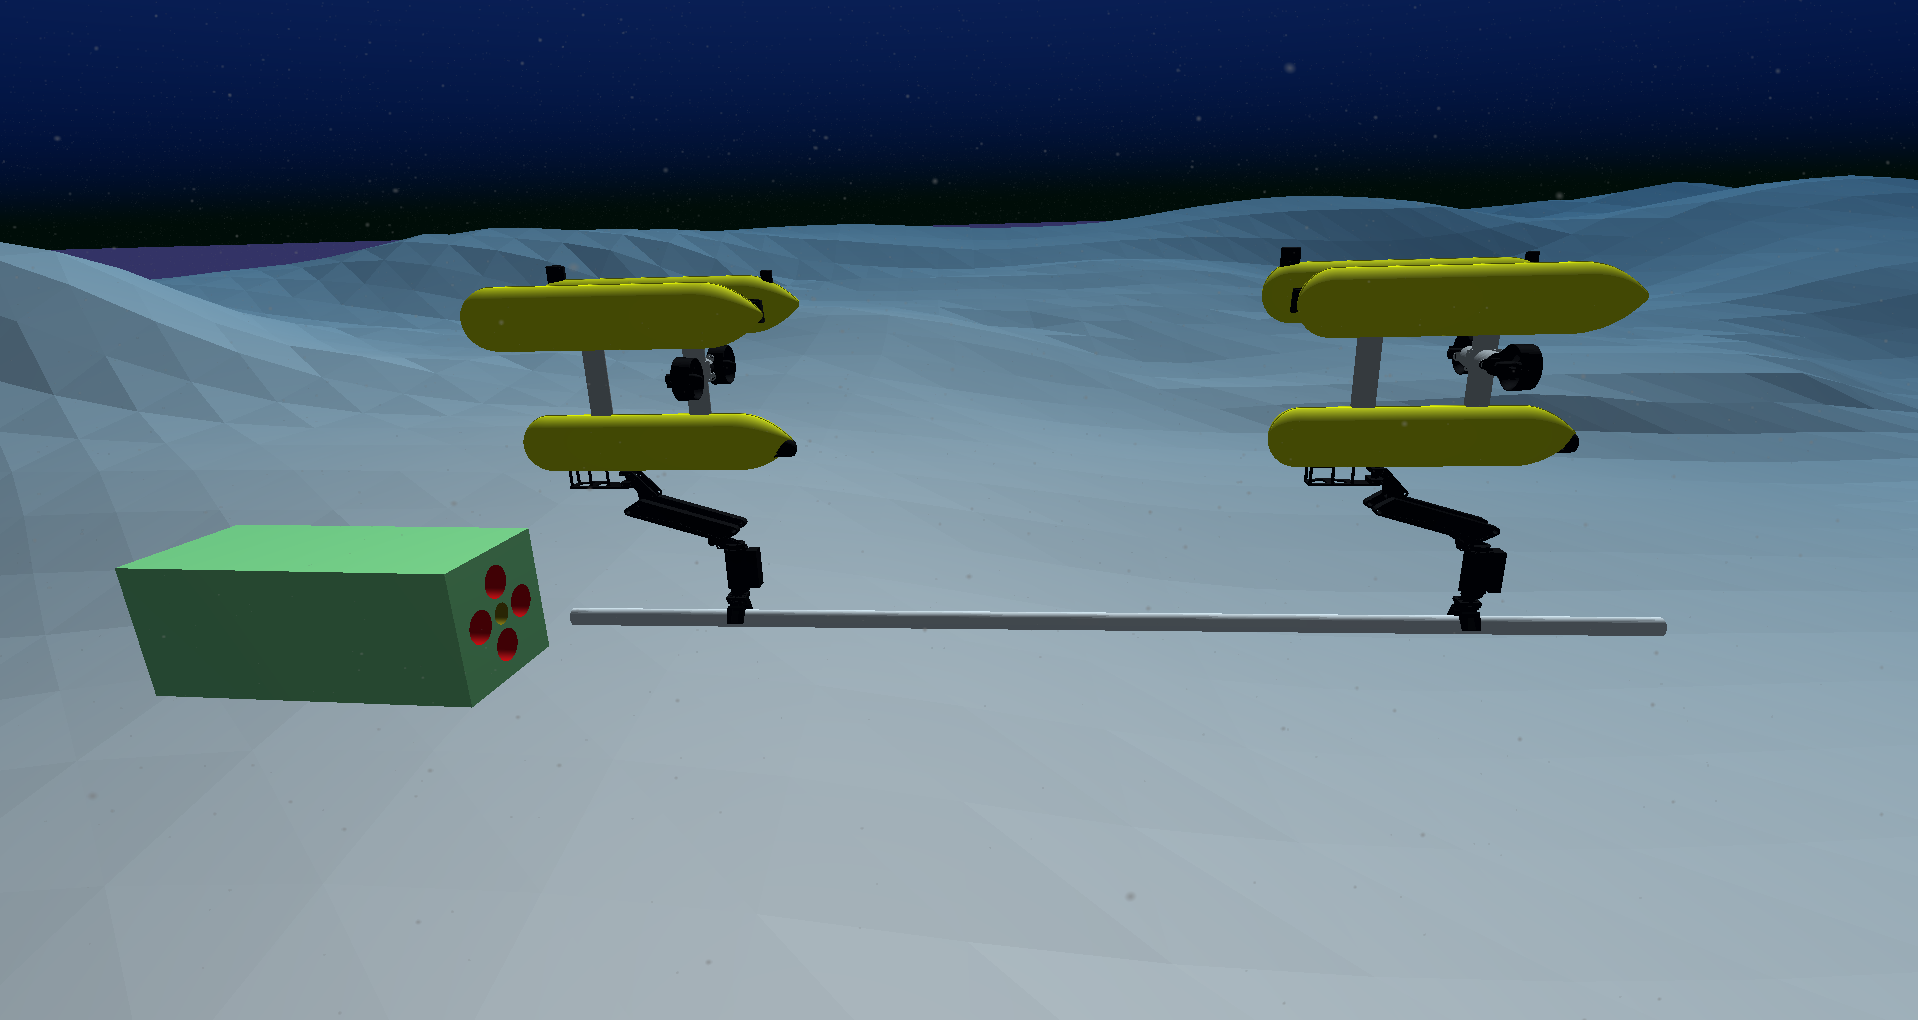
\includegraphics[width=10cm]{scenario_onlyTwin.png}
	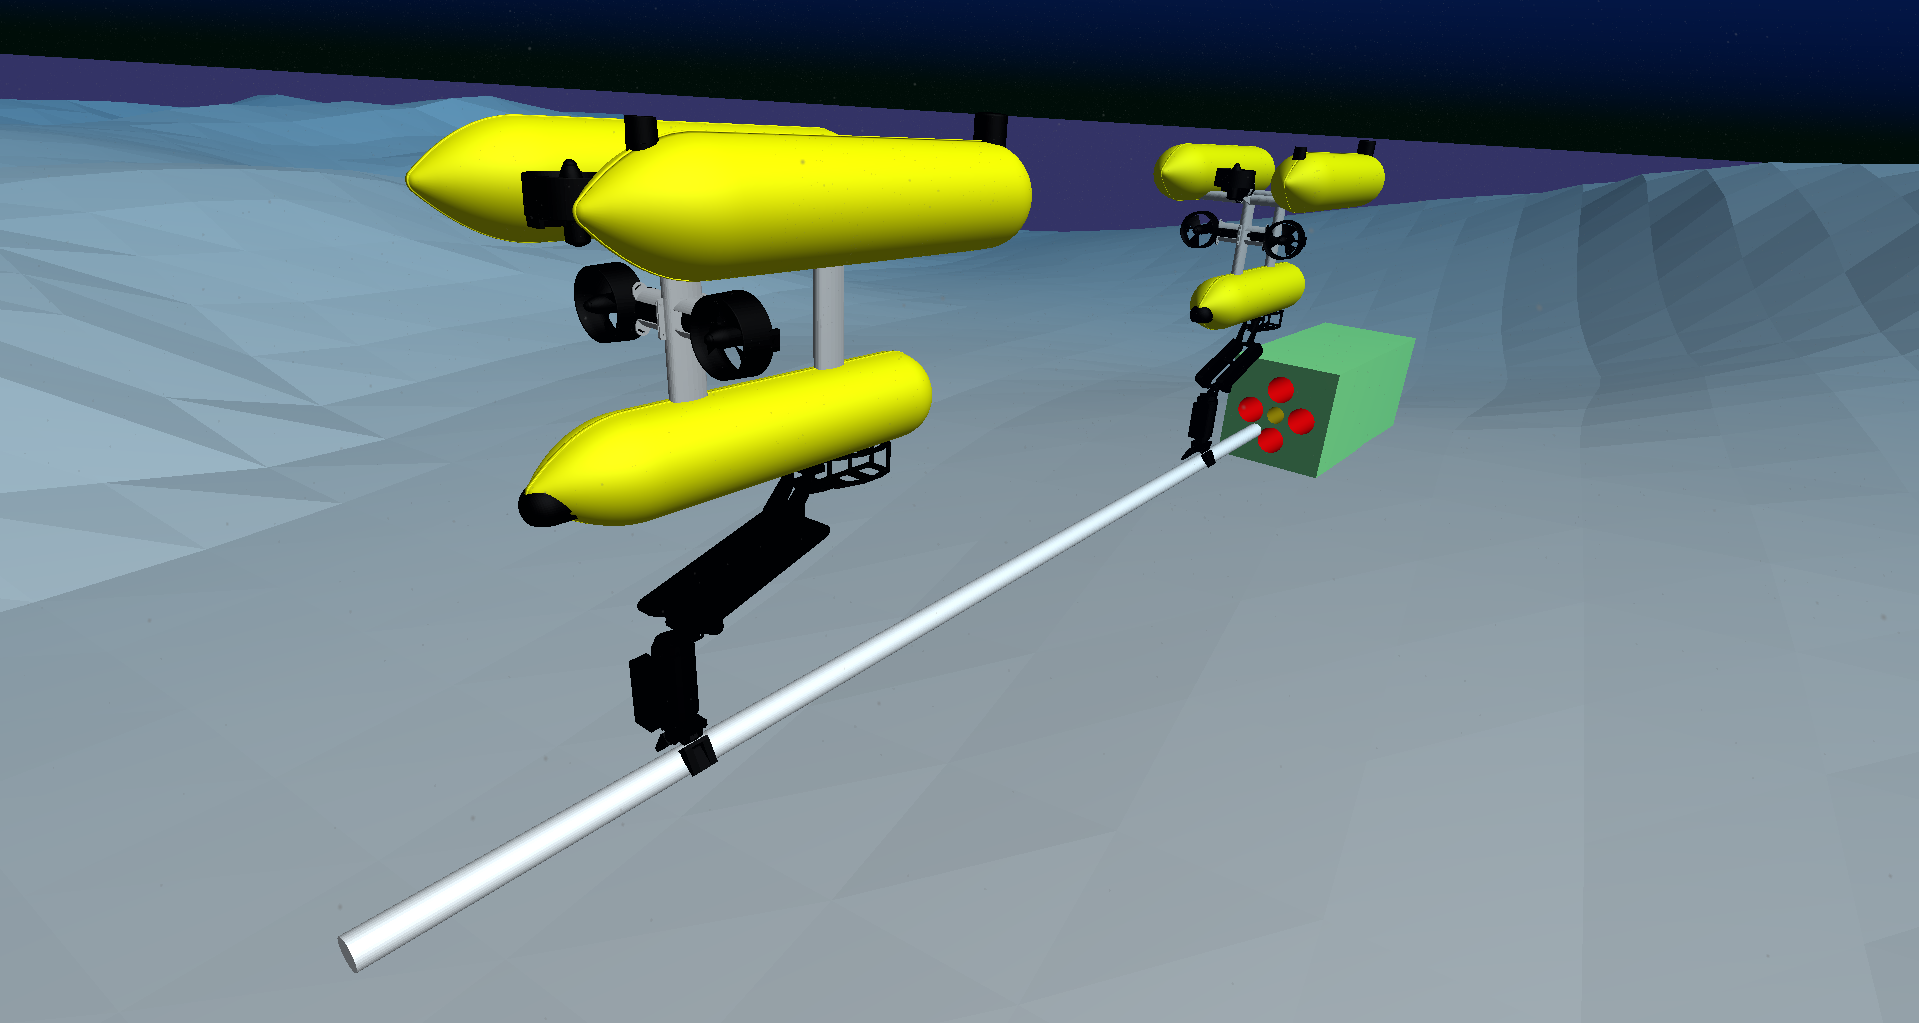
\includegraphics[width=10cm]{scenario_onlyTwin2.png}
	
	\caption[Scenario for test without the vision part]{Two differents angle view of the initial scenario for the results presented in this section. The pose estimation with vision is here neglected and the goal frame considered known without any errors.}
	\label{fig:onlyTwin_uwsim}
\end{figure}

